%! Graphentheoretische Konzepte und Algorithmen
%! Referat - Ausarbeitung
%! Adrian Helberg (ace346)
%! Start: 25.11.2019
%! Abgabe: 15.12.2016 20°°

% Preamble
\documentclass[11pt]{article}

% Packages
\usepackage[ngerman]{babel} % German Language Layout
\usepackage{geometry}
\usepackage{graphicx}
\usepackage{tocloft}
\usepackage{url}
\usepackage{xcolor}
\usepackage{listings}
\lstset{
backgroundcolor=\color{white},
basicstyle=\footnotesize,
breakatwhitespace=false,
breaklines=true,
captionpos=b,
commentstyle=\color{gray}\textit,
frame=tb,
keepspaces=true,
keywordstyle=\color{blue}\bfseries,
language=erlang,
numberstyle=\tiny\color{gray},
rulecolor=\color{black},
showspaces=false,
showstringspaces=false,
showtabs=false,
stepnumber=1,
stringstyle=\color{violet},
tabsize=2,
title=\lstname,
columns=fixed
}

\renewcommand{\cftsecleader}{\cftdotfill{\cftdotsep}} % ToC Dots
%\setcounter{tocdepth}{2} % ToC Depth Counter

\title{
\Large Graphentheoretische Konzepte und Algorithmen\\
\huge Referat - Ausarbeitung\\
\Large Aufgabe 3: Flu\ss{}probleme\\[0.3in]
}
\sub
\author{Adrian Helberg\\}
\date{\today}

\makeatletter
\def\@maketitle{
\linespread{2}
\raggedleft

\includegraphics[width=10cm]{../haw_logo.png}
\begin{center}
{\bfseries \sffamily \@title}
    Autor: {\@author}~\\
    Vortrag: 16.12.2019
\end{center}
\raggedright
\\~\\~\\~\\~\\~\\~\\~\\~\\~\\~\\~\\
Referat eingereicht im Rahmen der Vorlesung\\
Graphentheoretische Konzepte und Algorithmen\\~\\
im Studiengang Angewandte Informatik (AI)\\
am Department Informatik der Fakult\"at Technik und Informatik\\
der Hochschule f\"ur Angewandte Wissenschaften Hamburg\\~\\
Betreuender Pr\"ufer: Prof. Dr. C. Klauck\\
Abgegeben am \today
}
\makeatother

% Document
\begin{document}
    \maketitle
    \newpage
    \tableofcontents

    \newpage

    %%%%%%%%%%%%%%%%%%%
    %%% Einleitung %%%%
    %%%%%%%%%%%%%%%%%%%
    \section{Einleitung}

    \subsection{Flu\ss{}probleme}
    \textit{\"Ahnlich wie beim Problem des k\"urzesten Weges oder bei den elektrischen Netzwerken handelt es sich hier um eine der urspr\"unglichsten Aufgabenstellungen f\"ur Graphen, wo eben die Kanten als Verbindungen mit gewissen festen Eigenschaften wie L\"angen, Widerstand, etc. interpretiert werden.} \cite{alggra} (Seite 79, Kapitel 10)\\~\\
    Offensichtlich steht bei der genannten Problematik der Transport im Vordergrund, wobei die Durchflussmenge durch einen konstanten Wert begrenzt wird. Klassische Beispiele sind Verkehrs-Netze, Gleichstrom-Netzwerke und Abwassersysteme.

    \subsection{Laufzeitmessung}
    Ein Teil der Aufgabenstellung beinhaltet das Messen von Laufzeiten zur Analyse implementierter Algorithmen. Hierzu sind Testszenarien mit einem erwarteten Ergebnis zu erstellen und diese nachzuweisen. Weiter werden die sich ergebenen Laufzeiten nicht in Zeiteinheiten, sondern in der \textit{Landau-Notation} angegeben.

    %%%%%%%%%%%%%%%%
    %%% Kontext %%%%
    %%%%%%%%%%%%%%%%
    \section{Kontext}
    Hier ist die wissenschaftliche Vorarbeit zu einer gegebenen Aufgabenstellung gemeint. Hierzu geh\"ort die Recherche und Erarbeitung ben\"otigter Algorithmen und Thematiken.

    \subsection{Aufgabenstellung}\\
    Ziel der Aufgaben~\cite{gkapub} ist sowohl eine Implementierung zweier Algorithmen zum Finden des maximalen Durchsatzes (Flusses), als auch deren Vergleich und Analyse.\\~\\
    Folgende Algorithmen werden bearbeitet:
    \begin{itemize}
        \item[I.] Der Algorithmus von \textbf{Ford und Fulkerson} \footnote[1]{" `Ford-Fulkerson"', 1956, L.R.Ford \& D.R.Fulkerson}
        \item[II.] Der Algorithmus von \textbf{Edmonds und Karp} \footnote[2]{"`Edmonds-Karp"', 1970, Yefim Dinitz, 1972, J.Edmonds \& R.Karp}
    \end{itemize}\\~\\
    \underline{Zusatz}: Es soll nicht mittels Residualnetzwerks\footnote{Da es in der Aufgabenstellung um das Verstehen und Herausarbeiten verschiedener Strategien geht, wird ein weniger effizienter Algorithmus implementiert, als der mittels Residualnetzwerk, welcher intelligent die Markierung \"uber Vorw\"artskanten vornimmt} gearbeitet werden\\~\\
    Weitere Vorgaben:
    \begin{itemize}
        \item Ergebnisse sind nachvollziehbar:
        \begin{itemize}
            \item Ausgaben in Dateien
            \item Ausgabe auf dem Bildschirm
            \item Generierung von Graphen als Dot-Dateien und Bildern
        \end{itemize}
        \item Berechneter Fluss ist als Attribut an Kanten zu speichern (mittels interner Datenstruktur) zur Generierung von Flussgraphen als Bild
        \item Schnittstellen:
        \begin{itemize}
            \item fordfulkerson:fordfulkerson($<Filename>$,$<Quelle>$,$<Senke>$):\\ \indet [$<$Liste der im letzten Lauf inspizierten Ecken$>$]
            \item fordfulkerson:fordfulkersonT($<Graph>$,$<Quelle>$,$<Senke>$):\\ \indet [$<$Liste der im letzten Lauf inspizierten Ecken$>$]
            \item edmondskarp:edmondskarp($<Filename>$,$<Quelle>$,$<Senke>$):\\ \indet [$<$Liste der im letzten Lauf inspizierten Ecken$>$]
            \item edmondskarp:edmondskarpT($<Graph>$,$<Quelle>$,$<Senke>$):\\ \indet [$<$Liste der im letzten Lauf inspizierten Ecken$>$]
        \end{itemize}
        \item Erweiterung des abstrakten Datentyps "`adtgraph"' um eine Funktion \newline $printGFF(<Graph>,<Filename>)$ zur Erstellung von $*.dot$-Dateien aus gegebenen Graphen
        \begin{itemize}
            \item[!] \textbf{Entf\"allt hier, da der mitgelieferte abstrakte Datentyp "`adtgraph"' nur als Kompilat vorliegt und somit unver\"anderlich ist}
        \end{itemize}
        \item Nachweis der erwarteten Komplexit\"at durch Laufzeitmessung mittels bereitgestellter Module
        \item Gegebene Graphen sind zum Test der Korrektheit anzuwenden
        \item Logdateien zur Zeitmessung der Algorithmen sind anzulegen
        \item Bildschirmausgabe des Tests der Datei aufg3test.beam ist zu protokollieren
    \end{itemize}

    \subsection{Recherche}
    Graphen werden hier durch $G(V,E)$ mit $|V|$ Ecken und $|E|$ Kanten beschrieben.\\~\\
    Im Folgenden wird auf das Kapitel "`Flussprobleme"' aus dem Buch zur Vorlesung eingegangen~\cite{grbuch} (ab Seite 95).\\~\\
    $[\ldots]$ \textit{grunds\"atzlich mit schwach zusammenh\"angenden, schlichten gerichteten Graphen} $[\ldots]$\\~\\
    Ein Graph hei\ss{}t
    \begin{itemize}
        \item \textbf{zusammenh\"angend}, wenn die Knoten paarweise durch eine Kantenfolge verbunden sind
        \item \textbf{schwach zusammenh\"angend}, wenn der Graph, der entsteht, wenn man jede gerichtete Kante duch eine ungerichtete Kante ersetzt, zusammenh\"angend ist
        \item \textbf{schlicht}, wenn er ungerichtet ist und weder Mehrfachkanten, noch Schleifen besitzt
    \end{itemize}\\~\\
    $[\ldots]$ \textit{jede Kante gibt die Kapazit\"at $c(e\textsubscript{ij})=c\textsubscript{ij}$ der Kante an $[\ldots]$. Aus praktischen Gr\"unden nehmen wir dabei an, dass alle $c\textsubscript{ij}$ rationale Zahlen sind.}\\~\\
    In dieser Arbeit wird im Weiteren der Begriff \textbf{Netzwerk} verwendet, sollten Graphen die genannten Eigenschaften aufweisen.\\~\\
    \textbf{Definition 4.1} $[\ldots]$ \textit{Eine Kapazit\"at ist eine Funktion c, die jeder Kante $e\textsubscript{ij} \in E$  eine positive rationale Zahl ($> 0$) als Kapazi\"at zuordnet. Ein Fluss in $G$ von der Quelle $q = v\textsubscript{1}$ zu der Senke $s = v\textsubscript{n}$ ist eine Funktion $f$, die jeder Kante $e\textsubscript{ij} \in E$ eine nicht negative rationale Zahl zuordnet} $[\ldots]$\\~\\
    \underline{Notiz:} In einer Implementierung der Algorithmen kann $c$ als Kapazit\"at und $f$ als Fluss f\"ur Namen des jeweile Kantenattributs gesetzt werden.\\~\\
    Weiter gilt die
    \begin{itemize}
        \item \textbf{Kapazit\"atsbeschr\"ankung} ($e\textsubscript{ij}: f(e\textsubscript{ij} \leq c(e\textsubscript{ij})$) und
        \item die \textbf{Flusserhaltung} \\ ($\forall \textsubscript{j} \in \{1,\ldots n\}: \[ \sum_{e\textsubscript{ij} \in O(v\textsubscript{i}, e\textsubscript{ji} \in I(v\textsubscript{i}))} \] f(e\textsubscript{1j}) = \[ \sum_{} \] (f(e\textsubscript{ij}) - f(e\textsubscript{ji})) = 0$)
    \end{itemize}
    In dieser Arbeit wird im Weiteren der Begriff \textbf{Flussnetzwerk} verwendet, sollten Graphen diese Eigenschaften aufweisen $(V, E, f, c)$.\\
    Der Wert des \textbf{Flusses} $f$ mit $d = \[ \sum_{e\textsubscript{1j} \in O(q)} \] f(e\textsubscript{1j}) = \[ \sum_{e\textsubscript{in} \in I(s)} \] f(e\textsubscript{in})$ betr\"agt in den Ecken $q$ (Quelle) und $s$ (Senke) 0 [Null] (\textbf{Flusserhaltung}). Die maximale Menge, die von der Quelle zur Senke transportiert werden kann ist ein Fluss maximaler St\"arke.\\~\\
    \textbf{Definition 4.2} \textit{Ein Schnitt ist die Menge von Kanten $A(X,\bar X)$, wobei $q \in C$ und $s \in \bar X$.}\\~\\
    \textbf{Definition 4.3} \textit{Ein Fluss, dessen Wert} $min\{c(X,\bar X) \| A(X,\bar X)$ ist ein beliebiger Schnitt$\}$ \textit{entspricht hei\ss{}t ein \textbf{maximaler Fluss}.}\\~\\
    \textbf{Definition 4.4} \textit{Ein ungerichteter Weg von der Quelle q zur Senke s hei\ss{}t ein vergr\"u\ss{}ernder Weg, wenn gilt:}
    \begin{itemize}
        \item F\"ur jede Kante $e\textsubscript{ij}$ , die auf dem Weg entsprechend ihrer Richtung durchlaufen
        wird (sie wird als \textbf{Vorw\"artskante} bezeichnet), ist $f(e\textsubscript{ij}) < c(e\textsubscript{ij})$.
        \item F\"ur jede Kante $e\textsubscript{ij}$ , die auf dem Weg entgegen ihrer Richtung durchlaufen
        wird (sie wird als \textbf{R\"uckw\"artskante} bezeichnet), ist $f(e\textsubscript{ij}) > 0)$.
    \end{itemize}\\~\\
    \textbf{Satz 4.2} \textit{Wenn in einem Graphen G ein Fluss der St\"arke $d$ von der Quelle $q$ zur Senke $s$ flie\ss{}t, gilt genau eine der beiden Aussagen:}
    \begin{itemize}
        \item[1.] \textit{Es gibt einen vergr\"o\ss{}ernden Weg.}
        \item[2.] \textit{Es gibt einen Schnitt} $A(X,\bar X)$ \textit{mit} $c(X,\bar X) = d$.
    \end{itemize}\\~\\
    \underline{Notiz:} \textit{1.} kann bei einer Implementierung eine Rekursion ausl\"sen ("`Ein maximaler Fluss ist noch nicht gefunden"' - Erweiterbarkeit ist gegeben), wobei \textit{2.} die Abbruchbedingung beschreibt ("`Ein maximaler Fluss ist gefunden"' - Erweiterbarkeit nicht gegeben).\\~\\
    \textbf{Satz 4.3 (Max-flow-min-cut Theorem von Ford und Fulkerson)} \textit{In einem schwach zusammenh\"angendem schlichten Digraphen $G$ mit genau
    einer Quelle $q$ und genau einer Senke $s$ sowie der Kapazit\"atsfunktion $c$ und
    dem Fluss $f$ ist das Minimum der Kapazit\"at eines $q$ und $s$ trennenden Schnitts
    gleich der St\"arke eines maximalen Flusses von $q$ nach $s$.}

    \subsection{Komplexit\"at}
    Die Komplexit\"at des \textbf{Ford-Fulkerson} Algorithmus wird mit $O(|E| * d\textsubscript{max})$, mit $d\textsubscript{max}$ als Maximalwert von $d$, angegeben. Jede Kante muss maximal zweimal inspiziert\footnote{siehe Kapitel 3.1} werden (in jede Richtung einmal), um einen vergr. Weg zu finden (Worst-Case-Betrachtung). Die Inspektion ben\"otigt hier eine konstante Anzahl von Arbeitsschritten ($O(1)$). Ein neuer verg. Weg ist also nach jeweils $O(|E|)$ Schritten gefunden (wenn es einen gibt). Da maximal $d\textsubscript{max}$ vergr. Wege gefunden werden m\"ussen, ergibt sich eine Komplexit\"at von $O(|E| * d\textsubscript{max})$~\cite{grbuch} (Seite 105).\\~\\
    Weiter l\"asst sich der Speicherplatzbedarf der Eingabe durch $O(|V|\textsuperscript{2} * log(c\textsubscript{max}))$, mit $c\textsubscript{max}$ als Maximalwert der Kapazit\"aten aller Eckenpaare, absch\"atzen~\cite{grbuch} (Seite 105).\\~\\
    Der Algorithmus ist nicht polynomial, da der Arbeitsaufwand mit zunehmender Eingabe exponentiell ansteigt, weil $c\textsubscript{max} \leq d\textsubscript{max}$ verausgesetzt werden kann\footnote{Der Fluss steigt maximal bis $d$ an; deshalb sind Kapazit\"aten, die gr\"o\ss{}er als $d$ sind, vernachl\"assigbar} ($O(c\textsubscript{max}) = O(e\textsuperscript{log(c\textsubscript{max})})$)~\cite{grbuch} (Seite 106).\\~\\
    \textbf{Satz 4.4} \textit{Wenn jede Vergr\"o\ss{}erung der Flussst\"arke $d$ durch einen vergr. Weg minimaler Kantenanzahl erfolgt, dann sind h\"ochstens $O(|E| * |V|)$ vergr. Wege zu berechnen, bis $d$ seinen Maximalwert erreicht hat.}~\cite{grbuch} (Seite 106).\\~\\
    Satz 4.4 \"Andert den Algorithmus ab, damit die Problemgr\"o\ss{}e in Polynomialzeit anw\"achst.\\~\\
    Der \textbf{Edmonds-Karp} Algorithmus verbessert die Laufzeit des \textbf{Ford-Fulkerson}, welche $O(|E| * d\textsubscript{max})$ betr\"agt, zu einer Laufzeit von $O(|V| * |E|\textsuperscript{2})$, macht sie also unabh\"angig von $d\textsubscript{max}$. Da die Suchreihenfolge nach einem verg. Weg wohl definiert ist, resultiert dieser Algorithmus in einer geringeren Laufzeitkomplexit\"at.

    %%%%%%%%%%%%%%%%
    %%% Entwurf %%%%
    %%%%%%%%%%%%%%%%
    \section{Entwurf}
    Der Entwurf dient der allgemeinen Beschreibung der Vorg\"ange und der technischen Umsetzung als alleinige Vorlage, sodass eine Implementierung in beliebigen Programmiersparachen m\"oglich ist, ohne weitere Dokumente zu ben\"otigen. Sowohl die zu implementierenden Algorithmen als auch gewisse Datenstrukturen sind hier zu finden. So ist es m\"oglich auf bestimmte St\"arken und Schw\"achen von Programmiersprachen in diesem Kontext einzugehen, um so effiziente Softwarel\"osungen zu erstellen.\\~\\
    Beschreibungen von Schnittstellen sind hier jeweils f\"ur den fettgedruckten Teil gegeben und Beispiele f\"ur eine m\"ogliche Implementierung und Datenstrukturen sind f\"ur die funktionale und pr\"adikative Programmiersprache \textbf{Erlang}~\cite{erlwikipedia} verfasst, da sich die Aufgabenstellung auf eine Implementierung in \textbf{Erlang} bezieht.

    \subsection{Ford-Fulkerson}
    \textit{Der Algorithmus beruht auf der Idee, einen Weg von der Quelle zur Senke zu finden, entlang dessen der Fluss weiter vergr\"o\ss{}ert werden kann, ohne die Kapazit\"atsbeschr\"ankungen der Kanten zu verletzen.}~\cite{ffwikipedia} (Wirkungsprinzip)\\~\\
    Dieser Algorithmus baut im wesentlichen auf dem Beweis des Satzes 4.3 auf.

    \subsubsection{Algorithmus}
    Ecken des Graphen werden w\"ahrend der Suche nach einem vergr\"o\ss{}ernden (Abk\"irzung: vergr.) Weg mit $(+/-, Vorg\textsubscript{i}, \delta\textsubscript{i})$ markiert.
    \begin{itemize}
        \item $Vorg\textsubscript{i}$ beschreibt den Vorg\"anger von $v\textsubscript{i}$ auf einem vergr. Weg
        \item $\delta\textsubscript{i}$ gibt die bisher auf dem vergr. Weg maximal m\"ogliche \"Anderung der Flussst\"arke an
        \item $Vorg\textsubscript{i}$ wird mit einem Vorzeichen versehen, das angibt, ob eine Kante entsprechend ($+$) oder entgegen ($-$) ihrer Richtung durchlaufen wird
    \end{itemize}
    \newpage
    \underline{Algorithmus}:
    \begin{itemize}
        \item[1.] \textit{(Initialisierung) \\ Weise allen Kanten $f(e\textsubscript{ij})$ als einen (initialen) Wert zu, der die Nebenbedingungen erf\"ullt. Markiere $q$ mit $(undefiniert, \infty)$.}
        \item[2.] \textit{(Inpektion und Markierung)}
        \begin{itemize}
            \item[(a)] \textit{Falls alle markierten Ecken inspiziert wurden, gehe nach 4.}
            \item[(b)] \textit{W\"ahle eine beliebige markierte, aber noch nicht inspizierte Ecke v\textsubscript{i} und inspiziere sie wie folg (Berechnung des Inkrements)}
            \begin{itemize}
                \item[$\bullet$] \textit{(Vorw\"artskante) F\"ur jede Kante $e\textsubscript{ij} \in O(v\textsubscript{i})$ mit unmarkierter Ecke $v\textsubscript{j}$ und $f(e\textsubscript{ij}) < c(e\textsubscript{ij})$ markiere $v\textsubscript{j}$ mit $(+v\textsubscript{i},\delta\textsubscript{j})$, wobei $\delta\textsubscript{j}$ die kleinere der beiden Zahlen $c(e\textsubscript{ij}) - f(e\textsubscript{ij})$ und $\delta\textsubscript{i}$ ist.}
                \item[$\bullet$] \textit{(R\"uckw\"artskante) F\"ur jede Kante $e\textsubscript{ji} \in I(v\textsubscript{i})$ mit unmarkierter Ecke $v\textsubscript{j}$ und $f(e\textsubscript{ji}) > 0$ markiere $v\textsubscript{j}$ mit $(\−v\textsubscript{i}, \delta\textsubscript{j})$, wobei $\delta\textsubscript{j}$ die kleinere der beiden Zahlen $f(e\textsubscript{ji})$ und $\delta\textsubscript{i}$ ist.}
            \end{itemize}
            \item[(c)] \textit{Falls $s$ markiert ist, gehe zu 3., sonst zu 2.(a)}.
        \end{itemize}
        \item[3.] \textit{(Vergr\"o\ss{}erung der Flussst\"arke) \\ Bei $s$ beginnend l\"asst sich anhand der Markierungen der gefundene verg. Weg bis zur Ecke $q$ r\"uckw\"arts durchlaufen. F\"ur jede Verw\"artskante wird $f(e\textsubscript{ij})$ um $\delta\textsubscript{s}$ erh\"oht, und f\"ur jede R\"uckw\"artskante wird $f(e\textsubscript{ji})$ um $\delta\textsubscript{s}$ vermindert. Anschlie\ss{}end werden bei allen Ecken mit Ausnahme von $q$ die Markierungen entfernt. Gehe zu 2.}
        \item[4.] \textit{Es gibt keinen verg. Weg. Der jetzige Wert von $d$ ist optimal. Ein Schnitt $A(X,\bar X)$ mit $c(X,\bar X) = d$ wird gebildet von genau denjenigen Kanten, bei denen entweder die Anfangsecke oder die Endecke inspiziert ist.}
    \end{itemize}
    \underline{Notiz:} In Schritt \textit{1.} wird i.allg. $f(e\textsubscript{ij}) := 0$ f\"ur alle $i$ und $j$ gew\"ahlt.\\~\\
    Das Buch zur Vorlesung~\cite{grbuch}, aus dem die Arbeitsweise der Algorithmen entnommen wird, zeigt, wie der \textbf{Ford-Fulkerson} Algorithmus mithilfe einer Tabelle verarbeitet wird (ab Seite 103). Diese beschreibt zwei Zellen "`gekennzeichnete Ecke"' und "`Kennzeichnung"'. Erstere beinhaltet markierte Ecken, die mit "`*"' versehen werden sollten diese inspiziert werden, und die zweite Zelle zeigt die Markierung der Ecke.\\~\\
    \underline{Notiz:} Es bietet sich an f\"ur eine Implementierung eine \"ahnliche Datenstruktur beim Markieren zu w\"ahlen (z.B. Tupel). Das Inspizieren kann \"uber Attribute an Kanten gesetzt werden z.B. $\{+,18119,5\}$.

    \subsubsection{Schnittstelle}
    \textbf{fordfulkerson}:fordfulkerson($<Filename>$,$<Quelle>$,$<Senke>$):\\ \indet [$<$Liste der im letzten Lauf inspizierten Ecken$>$]
    \begin{itemize}
        \item \underline{Beschreibung}: Der \textbf{Ford-Fulkerson} Algorithmus ist in einem Arbeitspaket\\ "`fordfulkerson"' zu implementieren
        \item \underline{Beispiel}: Erlang-Modul
    \end{itemize}
\begin{lstlisting}
% The erlang file containing this code is named fordfulkerson.erl
-module(fordfulkerson).
% ...
\end{lstlisting}
    fordfulkerson:\textbf{fordfulkerson}($<Filename>$,$<Quelle>$,$<Senke>$):\\ \indet [$<$Liste der im letzten Lauf inspizierten Ecken$>$]
    \begin{itemize}
        \item \underline{Beschreibung}: Der Name in der Funktionssignatur ist fordfulkerson
        \item \underline{Beispiel}: Erlang-Funktion
    \end{itemize}
\begin{lstlisting}
% ...
fordfulkerson(...) -> ... .
% ...
\end{lstlisting}
    fordfulkerson:fordfulkerson($<$\textbf{Filename}$>$,$<Quelle>$,$<Senke>$):\\ \indet [$<$Liste der im letzten Lauf inspizierten Ecken$>$]
    \begin{itemize}
        \item \underline{Beschreibung}: Filename steht hier f\"ur den Namen der Datei, in der ein Graph gespeichert ist. Die Datei liegt im selben Verzeichnis, wie das Modul \textbf{fordfulkerson}
        \item \underline{Beispiel}: Dateiname als Erlang-Atom
    \end{itemize}
\begin{lstlisting}
% ...
fordfulkerson('graph01.graph', ...) -> ... .
% ...
\end{lstlisting}
    fordfulkerson:fordfulkerson($<Filename>$,$<$\textbf{Quelle}$>$,$<$\textbf{Senke}$>$):\\ \indet [$<$Liste der im letzten Lauf inspizierten Ecken$>$]
    \begin{itemize}
        \item \underline{Beschreibung}: Quelle und Senke geben an, wo die Fl\"usse berechnet werden. Fl\"usse flie\ss{}en von der Quelle bis zur Senke
        \item \underline{Beispiel}: Ganzzahlige Quelle und Senke
    \end{itemize}
\begin{lstlisting}
% ...
fordfulkerson(..., 1, 10) -> ... .
% ...
\end{lstlisting}
    fordfulkerson:fordfulkerson($<Filename>$,$<Quelle>$,$<Senke>$):\\ \indet [$<$\textbf{Liste der im letzten Lauf inspizierten Ecken}$>$]
    \begin{itemize}
        \item \underline{Beschreibung}: R\"uckgabe sind die letzten inspizierten Ecken des Algorithmus
        \item \underline{Beispiel}: Liste mit ganzzahligen Ecken
    \end{itemize}
\begin{lstlisting}
% ...
fordfulkerson(...) ->
Ecken = [1, 2, ...],
Ecken.
% ...
\end{lstlisting}

    \subsubsection{Datenstrukturen}
    Um \"Uberlegungen f\"ur die Datenstrukturen anzustellen, muss klar sein, wie auf Daten zugegriffen wird. Dazu wird der Algorithmus aus \textbf{Kapitel 3.1.1} untersucht.\\~\\
    \underline{Begriffserkl\"arungen}
    \begin{itemize}
        \item $<Graph>$ entspricht einer internen Datenstruktur aus \textbf{adtgraph}, welche beispielsweise mit $adtgrap:createG$, $adtgraph:importG$, etc. erstellt werden kann
        \item $<Node>$ bezeichnet eine Ecke eines Graphen, die auch mit einem Index versehen werden kann, sollten mehrere Ecken angesprochen werden (z.B. $<Node 1>$)
        \item $<Name>$ meint hier den Namen eines Attributs, das an einer Ecke oder einer Kante gesetzt werden kann
        \item $<Value>$ wird als Wert des Attributs gesetzt
        \item $<Vorzeichen>$ bezeichnet Vorw\"artskanten ($+$), R\"uckw\"artskanten ($-$), oder die Quell-Ecke ($/$)
        \item $<Vorg>$ ist der vorangegangene Knoten, der in der Markierung angegeben wird
        \item $<Delta>$ bezeichnet das im Algorithmus verwendete $\delta$
    \end{itemize}
    \newpage
    \underline{\"Uberlegungen zu Datenstrukturen zur Umsetzung des Algorithmus}\\~\\
    aus 1. \textit{(Initialisierung)}: Setzen von Werten aller Kanten
    \begin{itemize}
        \item Werte k\"onnen als Kantenattribut im ADT\footnote{abstrakter Datentyp} \textbf{adtgraph} gesetzt werden. Die Funktionalit\"at ist bereits gegeben und im Kompilat "`adtgraph.beam"' definiert. ($O(1)$)
\begin{lstlisting}
% Usage of adtgraph:setAtE function
adtgraph:setAtE(<Graph>,<Node1>,<Node2>,<Name>,<Value>).
% Example: adtgraph:setAtE({...},1,2,'flow',5).
\end{lstlisting}
        $<Node1>$ und $<Node2>$ formen hier eine Kante des Graphen $<Graph>$
        \item Um Werte \textit{aller} Kanten setzen zu k\"onnen, wird eine Funktionalit\"at gebraucht, die Kanten iteriert. ($O(N)$)\\
        Hier bietet es sich an eine Liste von Kanten mittels Rekursion zu iterieren
    \end{itemize}
    aus 2. \textit{(Inspektion und Markierung)}: \\~\\
    (a) \"Uberpr\"ufung auf Markierung und Inspektion
    \begin{itemize}
        \item Markiert wird mit Tuple $\{<Vorzeichen>,<Vorg>,<Delta>\}$ oder $nil$ als "`fehlende"' Markierung
        \item Inspiziert wird mit Atom: $'*'$ oder $nil$ als "`fehlende"' Inspektion
        \item Da eine Fallunterscheidung $A \&\& B$, mit $A$ als vorhandene Markierung und $B$ als vorhandene Inspektion, ben\"otigt wird, k\"onnen hier alle Knoten des Graphen rekursiv durchlaufen werden, um diese so auf Markierung und Inspektion zu \"uberpr\"ufen mittles Funktion "`getValV"' aus \textbf{adtgraph} ($O(N)$)
\begin{lstlisting}
% Usage of adtgraph:getValV function
adtgraph:getValV(<Graph>,<Node>,<Name>).
% Example: adtgraph:getValV({...},5,'Marke'). -> {'+',1,20}
\end{lstlisting}
    Attribute von Kanten k\"onnen \"uber die Funktion "`getValE"' aus \textbf{adtgraph} abgefragt werden ($O(1)$)
\begin{lstlisting}
% Usage of adtgraph:getValE function
adtgraph:getValE(<Graph>,<Node1>,<Node2>,<Name>).
% Example: adtgraph:getValE({...},1,2,'flow'). -> 20
\end{lstlisting}
    \end{itemize}
    (b) W\"ahlen einer beliebigen Ecke ($O(N)$), Vorw\"arts- und R\"uckw\"artskanten verarbeiten
    \begin{itemize}
        \item Um unabh\"angig von der gegebenen Datenstruktur aus \textbf{adtgraph} arbeiten zu k\"onnen, wird eine Liste \"uber alle Ecken des Graphen gemischt, um so eine \textbf{beliebige}, markierte, nicht inspizierte Ecke zu finden ($O(N)$)
\begin{lstlisting}
% Usage of util:shuffle function
util:shuffle(<List>).
% Example: util:shuffle([1,2,3,4]). -> [3,1,4,2]
\end{lstlisting}
        \item Inzidente Kanten der beliebig gew\"ahlten Ecke k\"onnen mithilfe der Funktion\\ "`getIncident"' aus \textbf{adtgraph} abgefragt werden ($O(1)$)
\begin{lstlisting}
% Usage of adtgraph:getIncident function
adtgraph:getIncident(<Graph>,<Node>).
% Example: adtgraph:getIncident({...},1). -> [1,2,1,3,4,1]
\end{lstlisting}
        \item Das Markieren der Kanten erfolgt \"ahnlich wie das Setzen von Attributen an Kanten
\begin{lstlisting}
% Usage of adtgraph:setAtE function
adtgraph:setAtE(<Graph>,<Node1>,<Node2>,<Name>,<Value>).
% Example: adtgraph:setAtE({...},1,2,'flow',5).
\end{lstlisting}
    \end{itemize}
    aus 3. \textit{Ver\"o\ss{}erung der Flussst\"arke}
    \begin{itemize}
        \item Die Aufgebenstellung gibt den Wert\\~\\ $[<$\textit{Liste der im letzten Lauf inspizierten Ecken}$>]$\\~\\ als R\"uckgabewert an. Darum ist es n\"otig die durchlaufenden Knoten zu halten. Dies kann \"uber eine Liste ($<Liste>$) geschehen
    \end{itemize}
    aus 4.
    \begin{itemize}
        \item Beim vorgegebenen R\"uckgabewert des Algorithmus ist es nicht n\"otig einen Schnitt (und damit $d$) zu berechnen. Hier m\"ussen keine \"Uberlegungen zu Datenstrukturen angestellt werden. Eine zu dieser Arbeit angefertige Inplementation kann schon nach Schritt 3 des Algorithmus terminieren und das Ergebnis zur\"uckliefern
    \end{itemize}
    \underline{Zusatz:}
    \begin{itemize}
        \item Das Einlesen von Graphen aus Dateien, kann \"uber "`importG"' aus \textbf{adtgraph} erfolgen
\begin{lstlisting}
% Usage of adtgraph:importG function
adtgraph:importG(<Filename>, <d/ud>).
% Example: adtgraph:importG('test', d). d for directed
\end{lstlisting}
    \end{itemize}

    \subsubsection{Ablauf}
    In der folgenden Abbildung ist der Ablauf der einzelnen Schritte im Gesamtkonzept des Algorithmus zu sehen.
    \begin{center}
        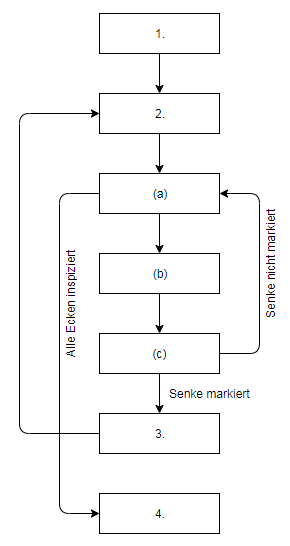
\includegraphics[height=12cm]{../fordfulkerson.PNG}
    \end{center}
    Dem Ablauf ist zu entnehmen, dass es sich anbietet den Algorithmus mittels zweier Schleifen zu implementieren:
    \begin{itemize}
        \item \"Au\ss{}ere Schleife ($2. \rightarrow 2a. \rightarrow 2b. \rightarrow 2c \rightarrow 3. \rightarrow 2 \rightarrow ...$) und
        \item Innere Schleife ($2a. \rightarrow 2b. \rightarrow 2c. \rightarrow 2a. \rightarrow ...$)
    \end{itemize}

    \subsubsection{Pseudocode}
    In diesem Abschnitt wird der Pseudocode f\"ur eine m\"ogliche Implementierung vorgestellt. Die Implementierung die der Aufgabenstellung zugrundeliegt, ist anhand dieses Codes erstellt worden. Wenn nicht anders angegeben, l\"auft der Algorithmus von Oben nach Unten durch
    \begin{itemize}
        \item[I.] Lese gerichteten Graphen $G$ aus Datei (Dateiname ist Inputparameter) ein. Setze den Fluss jeder Kante (rekursiv) des Graphen auf 0. (Attributname "`flow"'). Markiere Quell-Ecke (Inputparameter) mit $\{'/',undefined,'Infinity'\}$.\\~\\
        Anfang \textbf{\"Au\ss{}ere Schleife}:
        \item[II.] Pr\"ufe, ob alle markierten Ecken inspiziert sind. Wenn Ja gehe zu VI.. Frage Knotenliste des Graphen ab und mische diese, hole ersten Knoten dieser Liste. Inspiziere Knoten mit $'*'$. Hole alle inzidenten Kanten des Knotens und gehe diese wie folgt (rekursiv) durch.\\~\\
        Anfang \textbf{Innere Schleife}:
        \item[III.] Pr\"ufe auf vorhandene Markierung und fehlende Inspektion. Trifft eines der beiden nicht zu, wiederhole III. mit der n\"achsten Kante. Pr\"ufe Richtung der Kante. Markiere Knoten mit $\{<Richtung>,<Vorg>,<Delta>\}$ mit $<Vorg>$ als Knoten, der mit dem inspizierten Knoten die aktuelle Kante bildet und mit $<Delta>$ als Minimum aus $<Kapazit\"at>$ (Attributname "`weight"') $-$ $<Fluss>$ (Attributname "`flow"') und dem $<Delta>$ des Knotens. Sind noch nicht alle Kanten bearbeitet, gehe zu VIII mit der n\"achsten Kante.\\~\\
        Ende \textbf{Innere Schleife}
        \item[IV.] Pr\"ufe auf vorhandene Markierung des Senke-Knotens (Inputparameter). Fehlt die Markierung, gehe zu II.
        \item[V.] Gehe Markierungen (rekursiv) durch, beginnent mit dem Senke-Knoten, und setze den Fluss ("`flow"') der Kanten, die aus aktuellen Knoten und $<Vorg>$ der Markierung entsprechen, auf $Flow$ + $Delta$ der Markierung des Senke-Knotens. F\"uge bearbeitete Knoten der Knotenliste hinzu. Gehe zu II.\\~\\
        Ende \textbf{\"Au\ss{}ere Schleife}
        \item[VI.] Gib die Knotenliste zur\"uck.
    \end{itemize}

    \subsection{Edmonds-Karp}
    Der Algorithmus ist eine Modifikation des \textbf{Ford-Fulkerson} Algorithmus und bedarf deshelb nur wenige \"Anderungen im Entwurf und in einer Implementierung.

    \subsubsection{Algorithmus}
    Markierungen und Inspektionen erfolgen hier wie beim \textbf{Ford-Fulkerson} (Siehe Kapitel 3.1.1). Zur vereinfachung sind identische Teile beider Algorithmen weggelassen.\\~\\
    \underline{Algorithmus}
    \begin{itemize}
        \item[1.] \textit{(Initialisierung)}\\
        $\ldots$ \textit{Markiere $q$ mit $(undefiniert, \infty)$ und f\"uge $q$ der Queue hinzu.}
        \item[2.] \textit{(Inspektion und Markierung)}\\
        \textit{W\"ahle die n\"achste Ecke aus der Queue aus und inspiziere sie ...}
        \begin{itemize}
            \item \textit{Knoten, die markiert werden, werden der Queue hinzugef\"ugt; Knoten die inspiziert werden, werden der Queue entnommen}
        \end{itemize}
        \item[3.] $\ldots$ \textit{Anschlie\ss{}end werden bei allen Ecken mit Ausnahme von q die Markierungen entfernt und die Queue wird geleert, bis auf q. Gehe zu 2.}
    \end{itemize}

    \subsubsection{Schnittstelle}
    \textbf{edmondskarp}:edmondskarp($<Filename>$,$<Quelle>$,$<Senke>$):\\ \indet [$<$Liste der im letzten Lauf inspizierten Ecken$>$]
    \begin{itemize}
        \item \underline{Beschreibung}: Der \textbf{Edmonds-Karp} Algorithmus ist in einem Arbeitspaket\\ "`edmondskarp"' zu implementieren
        \item \underline{Beispiel}: Erlang-Modul
    \end{itemize}
\begin{lstlisting}
% The erlang file containing this code is named edmondskarp.erl
-module(edmondskarp).
% ...
\end{lstlisting}
    edmondskarp:\textbf{edmondskarp}($<Filename>$,$<Quelle>$,$<Senke>$):\\ \indet [$<$Liste der im letzten Lauf inspizierten Ecken$>$]
    \begin{itemize}
        \item \underline{Beschreibung}: Der Name in der Funktionssignatur ist edmondskarp
        \item \underline{Beispiel}: Erlang-Funktion
    \end{itemize}
\begin{lstlisting}
% ...
edmondskarp(...) -> ... .
% ...
\end{lstlisting}
    edmondskarp:edmondskarp($<$\textbf{Filename}$>$,$<Quelle>$,$<Senke>$):\\ \indet [$<$Liste der im letzten Lauf inspizierten Ecken$>$]
    \begin{itemize}
        \item \underline{Beschreibung}: Filename steht hier f\"ur den Namen der Datei, in der ein Graph gespeichert ist. Die Datei liegt im selben Verzeichnis, wie das Modul \textbf{edmondskarp}
        \item \underline{Beispiel}: Dateiname als Erlang-Atom
    \end{itemize}
\begin{lstlisting}
% ...
edmondskarp('graph01.graph', ...) -> ... .
% ...
\end{lstlisting}
    edmondskarp:edmondskarp($<Filename>$,$<$\textbf{Quelle}$>$,$<$\textbf{Senke}$>$):\\ \indet [$<$Liste der im letzten Lauf inspizierten Ecken$>$]
    \begin{itemize}
        \item \underline{Beschreibung}: Quelle und Senke geben an, wo die Fl\"usse berechnet werden. Fl\"usse flie\ss{}en von der Quelle bis zur Senke
        \item \underline{Beispiel}: Ganzzahlige Quelle und Senke
    \end{itemize}
\begin{lstlisting}
% ...
edmondskarp(..., 1, 10) -> ... .
% ...
\end{lstlisting}
    edmondskarp:edmondskarp($<Filename>$,$<Quelle>$,$<Senke>$):\\ \indet [$<$\textbf{Liste der im letzten Lauf inspizierten Ecken}$>$]
    \begin{itemize}
        \item \underline{Beschreibung}: R\"uckbage sind die letzten inspizierten Ecken des Algorithmus
        \item \underline{Beispiel}: Liste mit ganzzahligen Ecken
    \end{itemize}
\begin{lstlisting}
% ...
edmondskarp(...) ->
Ecken = [1, 2, ...],
Ecken.
% ...
\end{lstlisting}

    \subsubsection{Datenstrukturen}
    Um \"Uberlegungen f\"ur die Datenstrukturen anzustellen, muss klar sein, wie auf Daten zugegriffen wird. Dazu wird der Algorithmus aus \textbf{Kapitel 3.2.1} untersucht. Da sich dieser Algorithmus sehr \"ahnlich zum \textbf{Ford-Fulkerson} verh\"alt, wird dieses Kapitel stark abgek\"urzt. Siehe hierzu Kapitel 3.1.3\\~\\
    Da in der Aufgabenstellung spezifiziert ist, dass die Implementierung beider Algorithmen \textbf{Ford-Fulkerson} und \textbf{Edmonds-Karp} so \"ahnlich wie m\"oglich sein sollen, wird hier nur darauf eingegangen, dass eine Queue in Form einer Liste ($<List>$) beim \textbf{Edmonds-Karp} verwendet wird.

    \section{Laufzeitmessung}
    Dieses Kapitel stellt den Teil der Aufgabestellung dar, in dem Laufzeitmessungen f\"ur beide vorgestellten Algorithmen durchgef\"uhrt werden sollen, um somit die erwarteten Laufzeitkomplexit\"aten zu beweisen.

    \subsection{Versuchsaufbau}
    Um Laufzeitkomplexit\"aten erfassen zu k\"onnen, werden die Algorithmen mehrfach mit verschiedenen Eingabedaten ausgef\"uhrt. Somit kann untersucht werden, wie sich die Algorithmen verhalten (z.b. bei linear wachsenden Eingabedaten). Hierbei ist zu beachten, dass die zugrunde liegende Implementation in Erlang erstellt wurde und auf einem Windows-System ausgef\"uhrt wird. Je nach Auslastungen des Systems, auf dem die Algorithmen ausgef\"uhrt werden, k\"onnen ungenaue Messungen o.\"a. entstehen.\\~\\
    Zur Generieung von Inputdaten wird das Tool "`gengraph"' (\textbf{gengraph.beam}) genutzt:
\begin{lstlisting}
gengraph:gengraph(<Anzahl Ecken>,<minimaler Grad>,<Maximaler Grad>,<Min.Gewicht>,<Max.Gewicht,<Dateiname>).
% Example: gengraph:gengraph(100,3,5,1,100,'bsp').
\end{lstlisting}
    Das Beispiel zeigt, wie eine Generierung eines randomisierten Graphen mit 100 Ecken, einem minimalen Grad von 3, einem maximalen Grad von 5, einem Mindestgewicht von 1 und einem Maximalgewicht von 100 funktioniert. Mit derartigen Graphen werden beide Algorithmen ausgef\"uhrt und dann verglichen. Um eine m\"oglichst gute Wahl von Quell- und Senken-Knoten zu erlangen, wird die Knotenliste des generierten Graphen zuerst sortiert und dann das erste Element der sortierten Liste als Quelle und das letzte Elmenet als Senke genutzt. Der minimale Grad aller Knoten bel\"auft sich stets auf $|V|-1$, um so eine Vollvermaschung des Flussgraphen zu erreichen.

    \subsection{Parameter}
    Da in der Aufgabenstellung spezifiziert ist, dass das Tool \textbf{gengraph} zu verwenden ist, sind die Parameter f\"ur die Laufzeitmessung auf die Inputparameter des Tools beschr\"ankt.
    \begin{itemize}
        \item Anzahl Ecken
        \item minimaler Grad
        \item maximaler Grad
        \item Mindestgewicht
        \item Maximalgewicht
    \end{itemize}

    %%%%%%%%%%%%%%%%%%%%
    %%% Auswerttung %%%%
    %%%%%%%%%%%%%%%%%%%%
    \section{Auswertung}
    \begin{center}
        \begin{tabular}{c|c|c|c}
            \textbf{Edmonds-Karp} & \textbf{Ford-Fulkerson} & Anzahl Ecken & Anzahl Kanten\\
            \hline
            5 & 7 & 10 & 45\\
            22 & 25 & 20 & 190\\
            79 & 93 & 30 & 434\\
            217 & 232 & 40 & 780\\
            443 & 503 & 50 & 1225\\
            886 & 1001 & 60 & 1770\\
            1662 & 1896 & 70 & 2415\\
            2729 & 3072 & 80 & 3160\\
            5003 & 5144 & 90 & 4005\\
            8111 & 8785 & 100 & 4950\\
        \end{tabular}
    \end{center}
    \begin{center}
        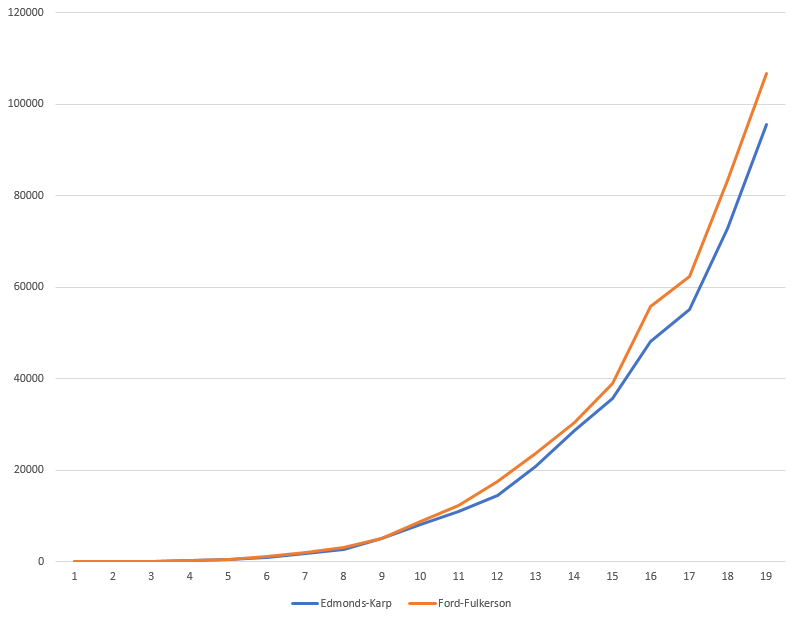
\includegraphics[height=8cm]{../auswertung.PNG}
    \end{center}
    Die Tabelle und der Graph zeigen, dass sich beide Algorithmen \"ahnlich verhalten bei linear steigender Anzahl Ecken, aber entgegen der Erwarteten Laufzeitkomplexit\"at exponentiell in der Laufzeit steigen.

    %%%%%%%%%%%%%%%%
    %%% Quellen %%%%
    %%%%%%%%%%%%%%%%
    \section{Quellen}
    \bibliographystyle{plain}
    \bibliography{quellen}
    \newpage

    %%%%%%%%%%%%%%%%%%
    %%% Erklärung %%%%
    %%%%%%%%%%%%%%%%%%
    \section{Erkl\"arung zur schriftlichen Ausarbeitung}

    Hiermit erkl\"are ich, dass ich diese schriftliche Ausarbeitung meines Referates selbstst\"andig und ohne fremde Hilfe verfasst habe und keine anderen als die angegebenen Quellen und Hilfsmittel benutzt habe sowie die aus fremden Quellen (dazu z\"ahlen auch Internetquellen) direkt oder indirekt \"ubernommenen Gedanken oder Wortlaute als solche kenntlich gemacht habe. Zudem erkl\"are ich, dass der zugeh\"orige Programmcode von mir selbst\"andig implementiert wurde ohne diesen oder Teile davon von Dritten im Wortlaut oder dem Sinn nach \"ubernommen zu haben. Die Arbeit habe ich bisher keinem anderen Pr\"ufungsamt in gleicher oder vergleichbarer Form vorgelegt. Sie wurde bisher nicht ver\"offentlicht.\\ \\ \\ \\
    Hamburg, den \today \indent\rule{8.5cm}{0.4pt}
\end{document}
